\documentclass[tikz,border=5]{standalone}
\usepackage{tikz}
\usetikzlibrary{calc, spy}
\makeatletter
\def\pgfpointnormalised#1{
\pgf@process{#1}
\pgfmathatantwo{\the\pgf@y}{\the\pgf@x}
\let\pgf@tmp=\pgfmathresult
\pgfmathcos@{\pgf@tmp}\pgf@x=\pgfmathresult pt\relax
\pgfmathsin@{\pgf@tmp}\pgf@y=\pgfmathresult pt\relax
}
\makeatother
\begin{document}
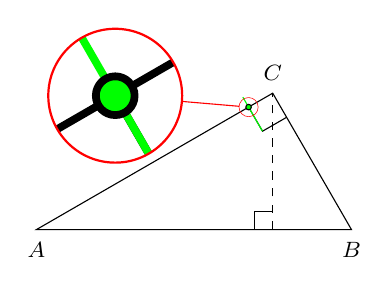
\begin{tikzpicture}[spy using outlines={circle, magnification=7, size=17mm, connect spies}]
\path (0,0) coordinate (A) ({(1/4)*16},0) coordinate (B) ({(1/4)*12},{(1/4)*(4*sqrt(3))}) coordinate (C);
\draw (A) -- (B) -- (C) -- cycle;
\node[anchor=north, inner sep=0, font=\footnotesize] at ($(A) +(0,-0.15)$){$A$};
\node[anchor=north, inner sep=0, font=\footnotesize] at ($(B) +(0,-0.15)$){$B$};
\node[anchor=south, inner sep=0, font=\footnotesize] at ($(C) +(0,0.15)$){$C$};
\coordinate (U) at ($(C)!5mm!45:(A)$);
\draw ($(A)!(U)!(C)$) -- (U) -- ($(B)!(U)!(C)$);
\draw[green] let \p1=($(B)-(C)$), \n1={atan(\y1/\x1)} in (U) -- ($(U) +({\n1+180}:0.5)$);
\draw[fill=green] ($(A)!(U)!(C)$) circle (1pt);
\coordinate (F) at ({(1/4)*(12)},0);
\draw[dashed] (F) -- (C);
\coordinate (V) at ($(F)!3.25mm!-45:(A)$);
\draw ($(A)!(V)!(B)$) -- (V) -- ($(C)!(V)!(F)$);
\spy[red] on ($(A)!(U)!(C)$) in node at (1,1.7);
\end{tikzpicture}
\end{document}